\documentclass[10pt,a4paper]{article}
\usepackage[italian]{babel}
\usepackage[T1]{fontenc}
\usepackage[utf8]{inputenc}
\usepackage[affil-it]{authblk}
\usepackage{lineno,hyperref}
\usepackage{amsmath}
\usepackage{amsfonts}
\usepackage{amssymb}
\usepackage{graphicx}
\usepackage{subcaption}


\newtheorem{remark}{Osservazione}
\newtheorem{definition}{Definizione}
\newtheorem{theorem}{Teorema}

\newcommand{\ww}{\mathbf{w}}
\newcommand{\vv}{\mathbf{v}}
\newcommand{\ee}{\mathbf{e}}
\newcommand{\ii}{\mathbf{i}}
\newcommand{\oo}{\mathbf{o}}

\begin{document}
\title{Appunti di Artificial Intelligence}

\author{Ivan Masnari%
  \thanks{e-mail: \texttt{ivan.masnari@studenti.unimi.it}}}
\affil{Facoltà di Informatica, UniMi, Milano}

\date{Ultima modifica: \today}
\maketitle
\section{Introduzione}

Dato un qualunque sistema, se disponiamo di un insieme di leggi o regole che lo descrivono completamente (nel caso di un sistema fisico avremmo delle equazioni differenziali) potremmo, in teoria, calcolarne in ogni momento lo stato e, quindi, prevederne l'evoluzione nel tempo. 
Tuttavia, nella vita di ogni giorno capita spesso di non avere a disposizione una conoscenza perfetta di un certo sistema. Tale informazione:
\begin{enumerate}
\item{può mancare.}
\item{possiamo averne una conoscenza approssimata.}
\end{enumerate}
L'intelligenza artificiale nasce con lo scopo di estrarre conoscenza direttamente dai dati in nostro possesso attraverso strumenti automatici. Questo modello si differenzia rispetto alla descrizione \emph{a priori} del sistema, in quanto lo simula per comprenderne \emph{a posteriori} il suo comportamento. Per far questo, è stato utile studiare come gli esseri viventi interagiscano con l'ambiente circostante e come vi si adattino.
Vari modelli di intelligenza artificiale sono stati proposti lungo la storia della disciplina. Una categorizzazione preliminare che si fa in letteratura è quella tra modelli:
\begin{itemize}
\item{\emph{simbolici}, in cui i dati vengono sottoposti a codifica e solo dopo manipolati. Storicamente questo è stato il primo approccio adottato (vedi sistemi esperti degli anni '70).}
\item{\emph{pre-simbolici}, in cui i dati vengono manipolati direttamente, senza la mediazione di una codifica. Fanno parte di questa famiglia: le reti neurali, i sistemi fuzzy e gli algoritmi evolutivi.}
\end{itemize}
Nel corso ci concentreremo sui secondi.

\section{Reti neurali}

\subsection{Background biologico}

Il nostro cervello ci permette di analizzare in maniera molto sofisticata l'ambiente in cui ci troviamo per agire nel miglior modo possibile (esempio: se riconosciamo un leone nella savana, scappiamo nell'altra direzione). Queste analisi sono basate sul funzionamento del cervello: come estrae informazioni, come queste interagiscono con l'informazioni contenute in memoria, etc. Lo studio di questi processi è un campo di ricerca molto attivo e multidisciplinare dove convergono gli interessi della biologia, della medicina e della psicologia.
Tali studi ci offrono dei modelli che simulano l'attività celebrale. Proprio questi modelli, vengono poi utilizzati dall'informatica per offrire strumenti di predizione, ottimizzazione e problem-solving in vari campi applicativi (guida automatizzata, smart cities, etc.). Il successo di questi modelli è condizionato dal fatto che il nostro cervello è un potente computer capace di computare in parallelo grandi porzioni di dati. Ma come funziona esattamente?

\begin{figure}
\centering
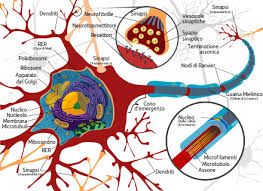
\includegraphics[scale=0.7]{img/neurone.jpeg}
\caption{Neurone}
\label{fig:1}
\end{figure}

Il cervello è composto da miliardi di cellule dette \emph{neuroni} (Figura \ref{fig:1}). Il neurone a sua volta è costituito da:
\begin{itemize}
\item{i \emph{dendriti}, i quali sono filamenti raggiunti dalle terminazioni di altri neuroni e che gli permettono di raccogliere informazioni grazie a processi biochimici originati dai così detti \emph{neurotrasmettitori}.}
\item{l'\emph{assone}: un lungo filamento che parte dal corpo centrale della cellula e trasmette segnali elettrici che, a loro volta, vanno ad attivare altri neuroni attraverso il rilascio di neurotrasmettitori.}
\end{itemize}

Quando e come il neurone trasmetta il segnale di attivazione dipende dal particolare modello fisiologico che si voglia adottare. Solitamente si considera un \emph{threshold}, superato il quale, l'assone viene depolarizzato e la differenza di potenziale provoca il passaggio di una corrente. Un diverso modello prende in considerazione non tanto la potenza dello stimolo quanto il loro numero. 
Questa struttura a network offre ottime prestazioni. Per un confronto con una CPU classica alleghiamo la seguente tabella:

\begin{figure}
\centering
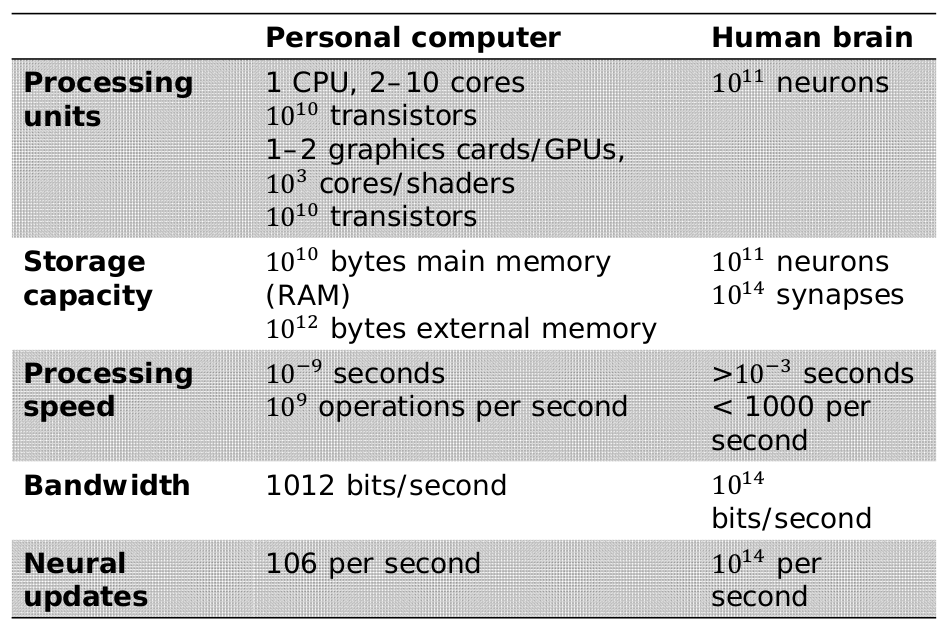
\includegraphics[scale=0.3]{img/cpuvshuman.png}
\end{figure}

\newpage

I vantaggi delle reti neurali sono:

\begin{enumerate}
\item{Alta velocità di calcolo, grazie al parallelismo.}
\item{Tolleranza ai guasti: la rete rimane funzionale anche quando molti neuroni smettono di funzionare.}
\item{La performance degrada in modo lineare con il numero di neuroni danneggiati.}
\item{Ottimo per l'apprendimento induttivo.}
\end{enumerate}

\subsection{Threshold logic unit}

Per implementare una rete neurale artificiale occorre trovare un analogo del neurone naturale. Tale compito è svolto dalle \emph{threshold logic unit}, nel seguito TLU. Una TLU è costituita da $n$ variabili di input $x_1 \dots x_n$ e un output $y$. Ad ogni unità viene assegnato un \emph{threshold} $\theta$ e ad ogni variabile di input un peso $w_i$ dove $i \in \{1, \dots ,n\}$ che rappresenta la rilevanza ai fine della computazione di quel particolare input.
L'output della TLU viene calcolato secondo la seguente formula:

\begin{equation}
y =  \begin{cases}
    1 & \text{se } \sum w_ix_i \geq \theta \\
    0 & \text{altrimenti} 
   \end{cases}
\end{equation}

Attraverso questo semplice meccanismo possiamo simulare alcune funzioni booleane. Se volessimo computare l'AND logico tra due input $x_1$ e $x_2$ basta assegnare valori ai pesi e al threshold in modo che soddisfino il seguente sistema di disequazioni:

\begin{equation}
	\begin{cases}
    w_1 + w_2 \geq \theta \\
    w_1 < \theta\\
    w_2 < \theta
   \end{cases}
\end{equation}

Risulta evidente che l'unica circostanza in cui l'output della TLU verrà posto ad 1 sarà quando entrambi gli input si trovano a 1. Inoltre, si noti che esistono varie scelte possibili di pesi e threshold che verificano le diseguaglianze.

\subsection{Interpretazione geometrica}

La condizione che calcola l'output della TLU somiglia molto da vicino all'equazione di un iperpiano (ovvero, un piano in $n$ dimensioni):

\begin{equation}
	 \sum w_ix_i + \theta = 0 
\end{equation}

Se pensiamo al caso precedente dell'AND logico e consideriamo i valori di input come coordinate in uno spazio bidimensionale, possiamo vedere che la retta definita da $x_1w_1 + x_2w_2 + \theta = 0$ corrisponde al confine che separa quelle combinazioni di valori che restituiscono come output 1 e quelle che, invece, restituiscono 0 (vedi Figura 2). \\
Da quanto detto, tuttavia, si può dedurre che una singola TLU potrà computare solo funzioni \emph{linearmente separabili}, ovvero funzioni in cui le coordinate associate agli input che restituiscono 1 possono essere separate da quelle che restituiscono 0 da una funzione lineare (punto, retta, piano o iperpiano a seconda della dimensione). 

\begin{figure}
\centering
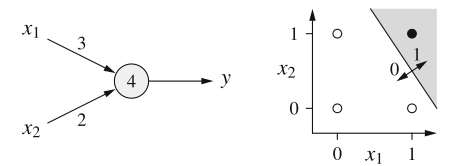
\includegraphics[scale=0.5]{img/geometria.png}
\caption{Rappresentazione geometrica della TLU per $x_1 \land x_2$}
\label{fig:2}
\end{figure}

\begin{definition}
Un insieme di punti $X$ in uno spazio euclideo si dice \emph{convesso} se e solo se non è vuoto, è connesso e ogni coppia di punti può essere congiunta da un segmento.
\end{definition}
\begin{definition}
Un \emph{guscio convesso} di un insieme di punti $X$ in uno spazio euclideo è il più piccolo insieme convesso che contiene $X$.
\end{definition}
\begin{theorem}
Due insiemi di punti $X$ e $Y$ si dicono linearmente separabili se e solo se i loro gusci convessi sono tra loro disgiunti.
\end{theorem}

Questo significa che già all'interno delle funzioni booleane ne esistono alcune che non possono essere simulate da una TLU. Come, per esempio, la doppia implicazione. Sebbene solo due funzioni booleane a due argomenti non siano linearmente indipendenti, al crescere degli argomenti il numero di funzioni che sono linearmente indipendenti diminuisce rapidamente. Per un numeri di argomenti arbitrariamente grande, una singola TLU non può calcolare "quasi" nessuna funzione.

\begin{figure}
\centering
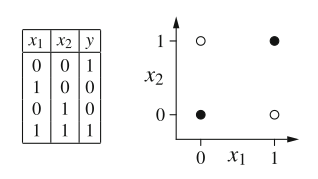
\includegraphics[scale=0.5]{img/doppiaimplicazione.png}
\caption{La doppia implicazione non è linearmente separabile}
\label{fig:3}
\end{figure}

Il problema può essere ovviato attraverso la costruzione di network di TLU più complessi. Come esempio consideriamo il network che simula la doppia implicazione (vedi figura \ref{fig:4}).

\begin{figure}
\centering
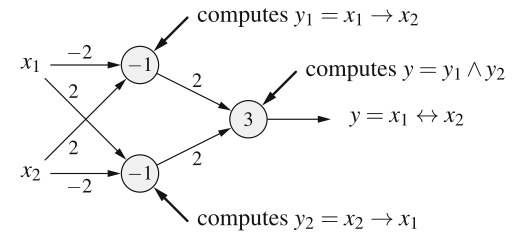
\includegraphics[scale=0.5]{img/netTLU.png}
\caption{network di TLU che simula la doppia implicazione}
\label{fig:4}
\end{figure}

\subsection{Training delle TLU}

L'interpretazione geometrica ci da una intuizione su come costruire una TLU avente 2 o 3 input, ma non è un metodo scalabile, nè automatizzato. Come far evolvere una TLU affinchè converga in modo autonomo ad una soluzione?
Un algoritmo che ci permette di automatizzare il processo è il seguente:

\begin{enumerate}
\item{Inizializzare i pesi e il threshold con valori randomici.}
\item{Determinare l'errore nell'output per un insieme di controlli. L'errore viene calcolato come una funzione dei pesi e del threshold $e(w_1,\dots,w_n,\theta)$.}
\item{Aggiornare i pesi e il threshold per correggere l'errore.}
\item{Iterare finchè l'errore si annulla.}
\end{enumerate}

Mostriamo il comportamento dell'algoritmo nel caso più semplice, in cui abbiamo un threshold ed un unico input (quindi, un unico peso associato). Poniamo che si voglia allenare il nostro neurone a calcolare la negazione booleana. Sia $x$ l'input, $w$ il peso associato e $\theta$ il threshold, allora l'output $y$ sarà definito come:

\begin{equation}
	y = \begin{cases}
    1 & \text{se } 0w = 0 \geq \theta \\
    0 & \text{se } 1w = w \geq \theta
   \end{cases}
\end{equation} 

Calcoliamo la funzione errore al variare di $w$ e $\theta$. Nel caso che $x = 0$ l'errore sarà 0 per un $\theta$ negativo e 1 per un $\theta$ negativo. Il peso non avrà alcuna influenza perchè viene annullato nella moltiplicazione con l'input. Quando, invece, $x = 1$, avremo che la funzione dipenderà da entrambi i parametri (vedi Figura \ref{fig:5}).

\begin{figure}
\centering
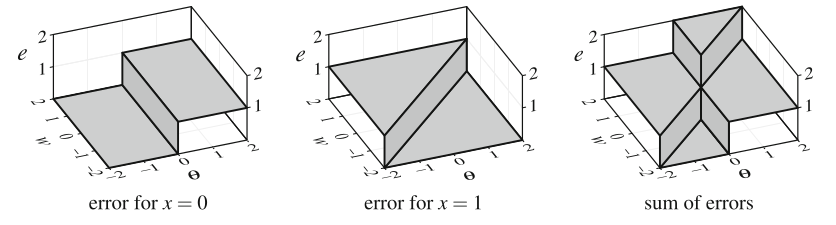
\includegraphics[scale=0.4]{img/error1.png}
\caption{funzione di errore per la negazione booleana}
\label{fig:5}
\end{figure}

La funzione di errore così calcolata non può essere usata direttamente nella nostra computazione perchè è composta da plateau e, quindi, non è ovunque derivabile. La soluzione è quella di calcolare la funzione di errore in modo tale che ci offra una misura di "quanto sbagliata" sia la relazione tra pesi e threshold. Otterremo così una funzione di errore che, seppur ancora non differenziabile, (vedi Figura \ref{fig:6}) lo sia localmente nei punti in cui l'errore si discosta da $0$. Ciò che faremo per correggere l'errore, dunque, sarà discendere verso l'area dove la funzione di errore si annulla. Questo è possibile esattamente perché abbiamo costruito una funzione derivabile nei punti in cui ci interessa, e cioè possiamo sempre calcolare la direzione migliore da prendere perchè si "scenda".
Ci sono due modi di immaginare il processo di allenamento del neurone:

\begin{itemize}
\item{\emph{Online learning}: dove correggiamo l'errore individualmente per ogni scelta dell'input.}
\item{\emph{Batch learning}: dove prendiamo in considerazione l'errore cumulato su una sequenza di input prima di applicare le correzioni.}
\end{itemize}

\begin{figure}
\centering
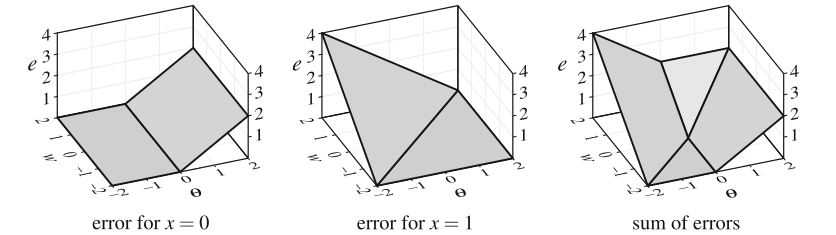
\includegraphics[scale=0.4]{img/error2.png}
\caption{funzione di errore differenziabile}
\label{fig:6}
\end{figure}

Definiamo di seguito la \emph{delta rule} o \emph{procedura di Widrow-Hoff} per allenare le TLU:

\begin{definition}
Sia $\vv$ = ($x_1, \dots, x_n$) il vettore di input di una TLU, \emph{o} l'output aspettato e \emph{y} il valore attuale. Se \emph{o} = \emph{y}, abbiamo finito. Al contrario, per ridurre l'errore computeremo nuovi valori per il threshold e i pesi nel seguente modo:
$$
\theta^{(new)} = \theta^{(old)} + \Delta\theta \text{ con } \Delta\theta = -\eta(\emph{o} - \emph{y})
$$
$$
\forall i \in \{1, \dots, n\}:w_i^{(new)} = w_i^{(old)} + \Delta w_i \text{ con } \Delta w_i = \eta(\emph{o} - \emph{y})x_i
$$
dove $\eta$ è il \emph{learning rate}. Più è alto, più i cambiamenti sui pesi e sui threshold sono drastici.

\end{definition}

Abbiamo visto prima, tuttavia, che non tutte le funzioni possono essere computate. Per le funzioni linearmente separabili esiste un teorema che ci garantisce che applicando la \emph{delta rule} l'algoritmo converga ad una soluzione.

\begin{theorem}
Sia $L = \{(\vv_1,\emph{o}_1), \dots, (\vv_n,\emph{o}_n)\}$ una sequenza di pattern di allenamento per la TLU, dove $\vv_i$ sono i vettori di input e $\emph{o}_i$ l'output atteso. 
Siano inoltre $L_0 = \{(\vv,\emph{o}) \in L | \emph{o} = 0\}$ e $L_1 = \{(\vv,\emph{o}) \in L | \emph{o} = 1\}$ rispettivamente gli insiemi delle coppie di pattern che hanno come output atteso 0 e quelle che hanno come pattern atteso 1. Se $L_0$ e $L_1$ sono linearmente separabili, allora esiste un $\ww$ vettore di pesi e un $\theta$ threshold t.c.:
$$
\forall (\vv,0) \in L_0: \ww\vv < \theta 
$$
$$
\forall (\vv,1) \in L_1: \ww\vv \geq \theta
$$
\end{theorem}

\begin{remark}
Negli esempi precedenti abbiamo codificato il valore booleano \emph{falso} come 0 e \emph{vero} come 1. Questa scelta non è felice perchè ha lo svantaggio che, nel caso di \emph{falso}, i pesi corrispondenti perchè la formula contiene l'input come fattore. Per evitare il problema si ricorre in letteratura ad una diversa codifica chiamata \emph{ADALINE} (ADAptive LINear Element), dove \emph{falso} viene ad assumere il valore $-1$ e il \emph{vero} $1$.
\end{remark}

Notiamo che questa procedura di allenamento vale solo per le singole TLU, ma abbiamo prima visto che le TLU possono computare solo funzioni linearmente separabili. Sebbene questo inconveniente si possa evitare prendendo in esame \emph{network} di TLU, questa procedura non si estende naturalmente a quel caso.

\subsection{Artificial neural network}

Un artificial neural network (in quello che segue ANN) può essere rappresentata come un grafo diretto $G = (U,C)$ dove i nodi sono TLU e gli archi sono le connessioni tra le varie unità. L'insieme dei nodi $U$ può essere partizionato in tre sottoinsiemi:

\begin{itemize}
\item{$U_{(in)}$: è l'insieme dei nodi di input, i quali ricevono in modo diretto l'informazione dall'ambiente.}
\item{$U_{(out)}$: è l'insieme dei nodi di output, i quali sono i soli nodi a comunicare con l'esterno.}
\item{$U_{(hidden)}$: è l'insieme dei nodi interni, i quali propagano la computazione.}
\end{itemize}

\begin{figure}
\centering
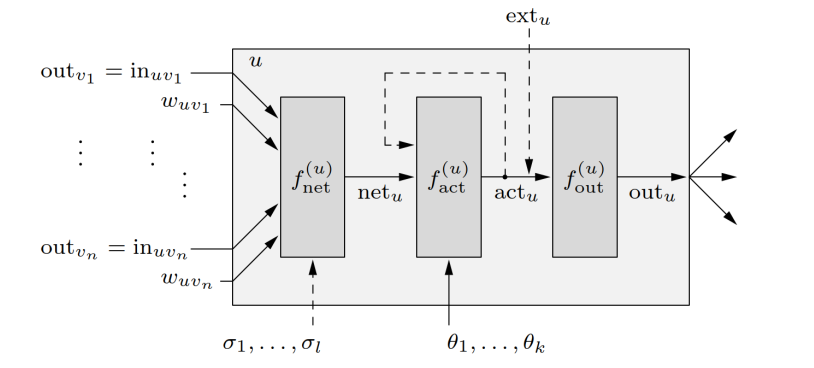
\includegraphics[scale=0.4]{img/ANN.png}
\caption{rappresentazione di un singolo neurone}
\label{fig:7}
\end{figure}

Ogni connessione $(u,v) \in C$ possiede un peso $w_{uv}$ che definisce l'importanza del dato originato da $v$ per il neurone $u$. Ad ogni neurone $u \in U$ vengono, invece, assegnate quattro variabili: il \emph{network input} $net_u$, la \emph{activation} $act_u$, l'\emph{output} $out_u$ e l'\emph{external input} $ext_u$ (vedi Figura \ref{fig:7}). Le prime tre variabili vengono calcolate in ogni momento dell'evoluzione dell'ANN grazie a tre funzioni associate:

\begin{enumerate}
\item{La \emph{network input function} $f^u_{net}$: calcola la somma pesata dell'input.}
\item{La \emph{activation function} $f^u_{act}$: ne esistono vari modelli (gaussiana, sigmoide, etc.) a seconda dell'applicazione.}
\item{La \emph{output function} $f^u_{out}$: definisce l'output a seconda che il neurone venga o meno attivato.}
\end{enumerate}

Se il grafo che rappresenta l'ANN è aciclico si parla di \emph{feed forward network} e la computazione procede in modo unidirezionale da $U_{(in)}$ a $U_{(out)}$ seguendo l'ordine topologico\footnote{L'ordine topologico è una numerazione dei vertici di un grafo diretto tale che tutti gli archi partano da un nodo associato ad un numero minore rispetto a quello associato al nodo di arrivo. Un ordine topologico esiste solo per grafi aciclici.} del network. Nel caso, invece, il grafo contenga un ciclo, allora si parla di \emph{recurrent network}.
I processi all'interno di un ANN si dividono in due fasi:

\begin{enumerate}
\item{La \emph{input phase}: dove gli input esterni vengono acquisiti dai neuroni di input.}
\item{La \emph{work phase}: dove i neuroni di input vengono spenti e un nuovo output viene computato da ogni neurone. La \emph{work phase} continua finchè gli output sono stabili o si raggiunge un timeout.}
\end{enumerate}

\begin{figure}
\centering
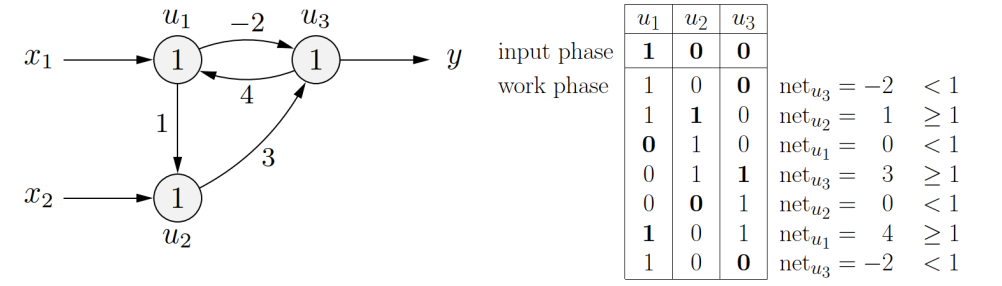
\includegraphics[scale=0.3]{img/rnn1.png}
\caption{computazione di una recurrent neural network che non giunge ad uno stato stabile}
\label{fig:8}
\end{figure}


Nel caso delle recurrent neural network, potrebbe accadere che non si giunga mai ad uno stato stabile a seconda di quale ordine di update dei neuroni si scelga di seguire. In Figura \ref{fig:8} abbiamo un esempio di una computazione con risultato oscillante in un recurrent neural network. L'ordine seguito per l'update è: $u_3,u_1,u_2,u_3,u_1,u_2\dots$. Se si fosse seguito un diverso ordine la computazione avrebbe raggiunto uno stato stabile.

\subsection{Training delle ANN}

Abbiamo visto in precedenza che è possibile allenare in modo automatico una singola TLU grazie alla delta rule. Come abbiamo già avuto modo di osservare questo procedimento non può essere generalizzato alle ANN. Tuttavia, i principi a cui ci ispiriamo sono i medesimi: calcolare correzioni ai pesi ed ai threshold dei singoli neuroni e aggiornarli di conseguenza. A seconda del tipo dei dati che utilizziamo per allenare le nostre ANN e dei criteri di ottimizzazione distiguiamo due tipi di apprendimento:

\begin{enumerate}
\item{\emph{fixed learning task} o apprendimento con supervisione}
\item{\emph{free learning task} o apprendimento senza supervisione}
\end{enumerate}

Nel caso di una fixed learning task avremo un insieme 
$L=\{(\ii_1,\oo_1),\dots,(\ii_n,\oo_n)\}$ di coppie che assegnano ad ogni input un output desiderato. Una volta completato il processo di apprendimento, la ANN dovrebbe essere in grado di restituire l'output adeguato rispetto all'input che le viene presentato. In pratica, questo accade raramente e bisogna accontentarsi di un risultato approssimativo.
Per giudicare in che misura una ANN si avvicina alla soluzione della fixed learning task si adotta una funzione di errore. Solitamente tale funziona viene calcolata come il quadrato della differenza tra l'output desiderato e quello attuale:
$$
e = \sum_{l \in L} \sum_{v \in U_{(out)}} e^l_v
$$
dove
$$
e^l_v = (o^l_v - out_v)^2
$$
è l'errore individuale per una particolare coppia $l$ e un neurone di output $v$. Il quadrato delle differenze viene scelto per vari motivi. Per prima cosa, errori positivi e negativi altrimenti si cancellerebbero a vicenda e non sarebbero presi in considerazione. In secondo luogo, questa funzione è ovunque derivabile, semplificando così il processo di aggiornamento dei pesi e dei threshold.
Nel free learning task avremo, invece, solo una sequenza di input $L = \{\ii_1, \dots, \ii_n\}$. Questo comporta che, a differenza del fixed learning task, non avremo modo di calcolare una funzione di errore rispetto ad un output atteso. In linea di principio, infatti, l'obiettivo di un free learning task sarà quello di produrre un output "simile" per input "simili". Un caso particolare potrebbe essere quello del \emph{clustering} dei vettori di input. 
Qualsiasi processo di apprendimento si scelga esistono alcune buone pratiche che è utile seguire. Una è quella di normalizzare il vettore di input. Comunemente lo si scala in modo tale che abbia media uguale a 0 e la varianza ad 1. Per fare questo uno deve calcolare per ogni neurone $u_k \in U_{(in)}$ la media aritmetica $\mu_k$ e la deviazione standard $\sigma_k$ degli input esterni:

$$
\mu_k = \frac{1}{|L|}\sum_{l \in L} ext^l_{u_k} \quad \quad \sigma_k = \sqrt{\frac{1}{|L|}\sum_{l \in L} (ext^l_{u_k} - \mu_k)^2}
$$

Quindi gli input esterni vengono ricalcolati secondo questa formula:

$$
ext^{new}_{u_k} = \frac{ext^{old}_{u_k} - \mu_k}{\sigma_k}
$$

\subsection{Multi-layer perceptrons}

\begin{figure}
\centering
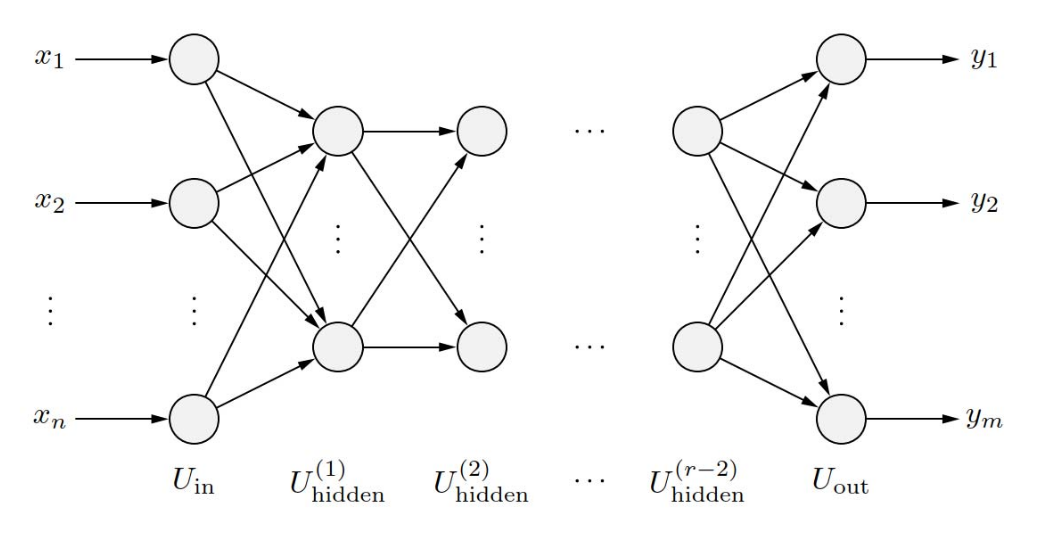
\includegraphics[scale=0.3]{img/MLP.png}
\caption{multi-layer perceptrons}
\label{fig:9}
\end{figure}


Una delle prime ANN sviluppate furono i \emph{multi-layer perceptrons} (nel seguito MLP). Le MLP sono particolari feed-forward network  in cui le unità base (i percettroni) sono organizzati in \emph{layer} e ogni layer ha connessioni solo con il layer successivo (vedi Figura \ref{fig:9}). Questo permette di minimizzare il fenomeno delle continue ricomputazioni che avverrebbero durante la propagazione del segnale nei normali feed-forward network.
La network input function di ogni neurone $u \in U_{(hidden) \cup U_{(out)}}$ viene calcolata come la somma pesata degli input, come:
$$
f^u_{net}(\ww_u,\ii_u) = \sum_{v \in pred(u)} w_{uv}out_v
$$
L'activation function, invece, è una così detta \emph{funzione sigmoide}, ossia una funzione monotona non descrescente tale che:
$$
f: \mathbb{R} \to [0,1] \quad \text{ con } \lim_{x\to-\infty}f(x) = 0 \quad \text{ e } \lim_{x\to\infty}f(x) = 1
$$

\begin{figure}

\begin{subfigure}{0.5\textwidth}
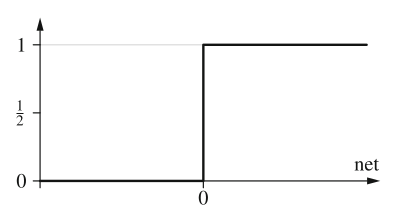
\includegraphics[width=0.9\linewidth, height=3cm]{img/step.png} 
\caption{step function}
\end{subfigure} %%
\begin{subfigure}{0.5\textwidth}
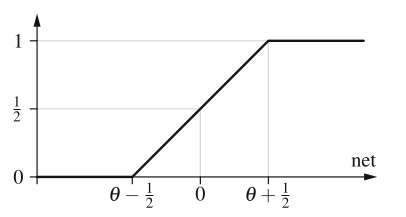
\includegraphics[width=0.9\linewidth, height=3cm]{img/semilinear.png}
\caption{semi-linear function}
\end{subfigure} 
\begin{subfigure}{0.5\textwidth}
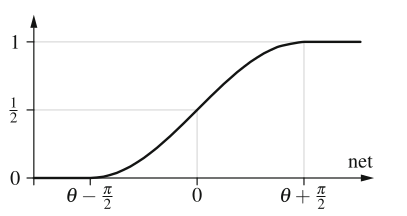
\includegraphics[width=0.9\linewidth, height=3cm]{img/sineup.png} 
\caption{sine up to saturation}
\end{subfigure}
\begin{subfigure}{0.5\textwidth}
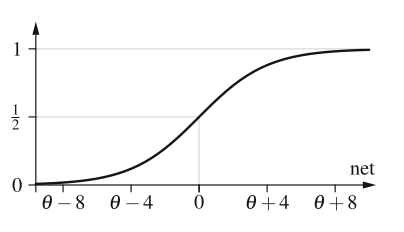
\includegraphics[width=0.9\linewidth, height=3cm]{img/logistic.png} 
\caption{logistic function}
\end{subfigure}


\caption{Alcune funzioni sigmoidi}
\label{fig:10}
\end{figure}

La funzione di output può essere sia una sigmoide oppure una semplice funzione lineare. \\
La struttura a layer di un MLP suggerisce che si possa descrivere il network con l'aiuto di una matrice dei pesi. In questo modo la computazione del MLP può essere rappresentata attraverso la moltiplicazione tra matrici e vettori. Tuttavia, noi non abbiamo utilizzato in classe una matrice per l'intero network, ma una per ogni singolo layer. Siano $U_1 = \{ v_1, \dots, v_n \}$ e $U_2 = \{ u_1, \dots, u_m \}$ due layer consecutivi di neuroni. I pesi delle loro connessioni sono codificati in una matrice $W$ di dimensioni $n \times m$:

$$
W = \begin{pmatrix}
  w_{u_1v_1} & w_{u_1v_2} & \cdots & w_{u_1v_n} \\
  w_{u_2v_1} & w_{u_2v_2} & \cdots & w_{u_2v_n} \\
  \vdots  & \vdots  & \ddots & \vdots  \\
  w_{u_mv_1} & w_{u_mv_2} & \cdots & w_{u_mv_n} 
 \end{pmatrix}
$$

Se due neuroni $u_i$ e $v_j$ non sono connessi, è sufficiente porre $w_{u_iv_j} = 0$. Il vantaggio di questa matrice sta nel fatto che è possibile scrivere il network input di un layer come:

$$
\mathbf{net}_{U_2} = W \mathbf{in}_{U_2} = W \mathbf{out}_{U_1}
$$

dove $\mathbf{net}_{U_2} = (net_{u_1}, \dots, net_{u_m})^\top$ e $\mathbf{in}_{U_2} = \mathbf{out}_{U_1} = (out_{v_1}, \dots, out_{v_n})^\top$. \\
Fino ad adesso abbiamo visto che le ANN possono rappresentare funzioni booleane, ma quando si parla di funzioni a valori continui? 


\begin{theorem}
Ogni funzione Riemann-integrabile è approssimata con precisione arbitraria da un MLP avente quattro layer.
\end{theorem}

\begin{figure}
\centering
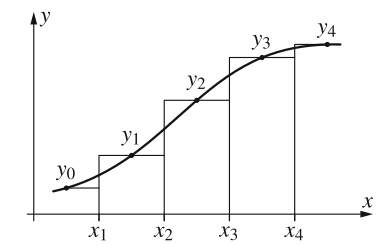
\includegraphics[scale=0.4]{img/approx.png}
\caption{Approssimazione di una funzione continua con una step function}
\label{fig:11}
\end{figure}

\begin{figure}
\centering
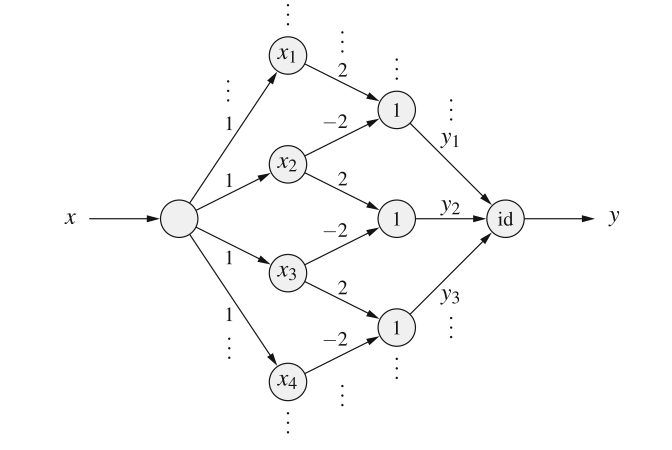
\includegraphics[scale=0.3]{img/riemann.png}
\caption{MLP che calcola la step function in Figura \ref{fig:11}}
\label{fig:12}
\end{figure}

Ogni funzione, infatti, può essere approssimata da una step function (come in Figura \ref{fig:11}). Ad ogni pivot $x_i$ associamo nel nostro MLP un neurone nel primo hidden layer (vedi Figura \ref{fig:12}). Nel secondo hidden layer creiamo un neurone per ogni scalino, il quale riceverà input dai due neuroni del primo livello che sono assegnati ai valori $x_i$ e $x_{i+1}$ che definiscono i bordi dello scalino. A questo punto, scegliamo pesi e threshold in modo tale che il neurone venga attivato se e solo se l'input è maggiore di $x_i$ e minore di $x_{i+1}$. Siccome la funzione di attivazione del neurone di output è la funzione di identità, il valore così calcolato viene emesso così come è ricevuto. 
Dovrebbe essere chiaro che l'approssimazione può crescere a piacere semplicemente aggiungendo neuroni e diminuendo la lunghezza dei gradini. Possiamo, inoltre, risparmiarci un layer se non utilizziamo nel calcolo l'altezza assoluta ma quella relativa come peso della connessione al neurone di output.
Bisogna notare, comunque, che questo risultato non ha natura costruttiva, ossia non ci dice come deve essere fatto un MLP che approssimi con una data accuratezza una certa funzione. Tutto ciò che afferma il Teorema 3 è che limitare il numero di layer non pregiudica la proprietà del MLP di essere un \emph{approssimatore universale}.

\subsection{Regressione}

Abbiamo visto che per allenare un ANN occorre minimizzare la funzione di errore, la quale si calcola solitamente come il quadrato della differenza tra output aspettato e attuale. Questo avvicina il problema dell'apprendimento nelle reti neurali a quello più generale della \emph{regressione}. La regressione è una tecnica molto usata in analisi e in statistica per estrapolare la retta (o, più in generale, il polinomio) che meglio approssima la relazione esistente in un insieme di dati/osservazioni. Detto in modo più formale, se $G = \{(\ww_0,y_0), \dots, (\ww_n,y_n)\}$ è il nostro dataset e immaginiamo esista una relazione funzionale tra il vettore di input $\ww_i$ e l'ascissa $y$, allora la regressione ci aiuterà a trovare i parametri di quella funzione. A seconda del diverso genere di funzione avremo diverse forme di regressione.

\subsubsection{Regressione lineare}

Se ci aspettiamo che le nostre due quantità $x$ e $y$ esibiscano una dipendenza lineare, allora dovremo identificare i parametri $a$ e $b$ che individuano la retta $y = g(x) = a + bx$. In generale, tuttavia, non sarà possibile trovare una singola retta che passi per tutti i punti del nostro dataset. Quello che faremo sarà trovare la retta che devi dai punti il meno possibile e che, quindi, minimizzi l'errore calcolato come segue: 

$$
F(a,b) = \sum(g(x_i) - y_i)^2 = \sum(a + bx_i - y_i)^2
$$

Il teorema di Fermat ci dice che una condizione necessaria perchè un minimo della funzione $F(a,b)$ esista è che la derivata parziale in entrambi i parametri si annulli:

$$
\frac{\partial F}{\partial a} = \sum 2(a + bx_i - y_i) = 0
$$

$$
\frac{\partial F}{\partial b} = \sum 2(a + bx_i - y_i)x_i = 0
$$

Questo sistema può essere risolto con alcune semplici tecniche di algebra lineare (vedi pag. 174 del libro). La soluzione così trovata sarà unica a meno che ogni valore $x_i$ sia identico. 

\subsubsection{Regressione polinomiale e multilineare}

Il metodo precedente può essere esteso in modo ovvio a polinomi di ordine arbitrario. In questo caso, si prende come ipotesi che la funzione indotta dal dataset approssimi un polinomio di ordine $n$:

$$
y = p(x) = a_o + a_1x + \dots + a_nx^n
$$

E si cercherà di minimizzare la funzione $F$ tale che:

$$
F(a_1,\dots,a_n) = \sum(p(x_i) - y_i)^2 = \sum(a_o + a_1x + \dots + a_nx^n -y_i)^2
$$

Come nel caso della regressione lineare, la funzione potrà essere minimizzata solo se le derivate parziali rispetto ai parametri $a_i$ si annullano:

$$
\frac{\partial F}{\partial a_1} = 0 \quad \dots \quad \frac{\partial F}{\partial a_n} = 0
$$

Inoltre, non siamo limitati a calcolare funzioni ad un solo argomento. Con alcune minori modifiche questo metodo è capace di approssimare funzioni in un numero arbitrario di argomenti. In quel caso, la chiameremo \emph{regressione multilineare}.

\subsubsection{Regressione logistica}

Nel situazione in cui il nostro dataset non sia approssimato con sufficiente accuratezza da una funzione polinomiale, potremmo dover utilizzare funzioni di generi diversi. Data, per esempio, una funzione della forma:

$$
y = ax^b
$$

possiamo trasformarla in una equazione lineare applicando l'operazione di logaritmo:

$$
ln(y) = ln(a) + bln(x)
$$

Nel caso delle ANN ci interessiamo in particolare alla funzione logistica (vedi Figura \ref{fig:10}(d)):

$$
y = \frac{Y}{1 + e^{a+bx}}
$$

Siccome molte ANN utilizzano come funzione di attivazione del neurone proprio la funzione logistica, se trovassimo un modo di applicarci il metodo della regressione potremmo determinare i parametri di qualsiasi network a due layer con un unico input. Il valore $a$ nella funzione corrisponderebbe al threshold del neurone di output e la $b$ al peso dell'input. Possiamo "linearizzare" la funzione logistica applicandoci le seguenti trasformazioni (comunemente chiamata \emph{logit transformation}):

$$
y = \frac{Y}{1 + e^{a+bx}} \leftrightarrow \frac{1}{y} = \frac{1 + e^{a+bx}}{Y} \leftrightarrow \frac{Y - y}{y} = e^{a+bx}
$$

Se estendiamo il nostro approccio fino a comprendere funzioni con più argomenti, in analogia a quanto accade nella regressione multilineare, possiamo utilizzarlo per computare i pesi di network a due layer con arbitrari neuroni di input. Tuttavia, siccome il metodo della somma degli errori funziona solo quando parliamo di neuroni di output, questo approccio non può essere esteso a network con più di due layer.


\section{Sistemi fuzzy}


\section{Algoritmi evolutivi}


\end{document}